\subsection{ARFC Research Group}
\begin{frame}
  \frametitle{Advanced Reactors and Fuel Cycles group (PI: Kathryn Huff)}
               \begin{figure}[t]
                \vspace*{-0.1in}
                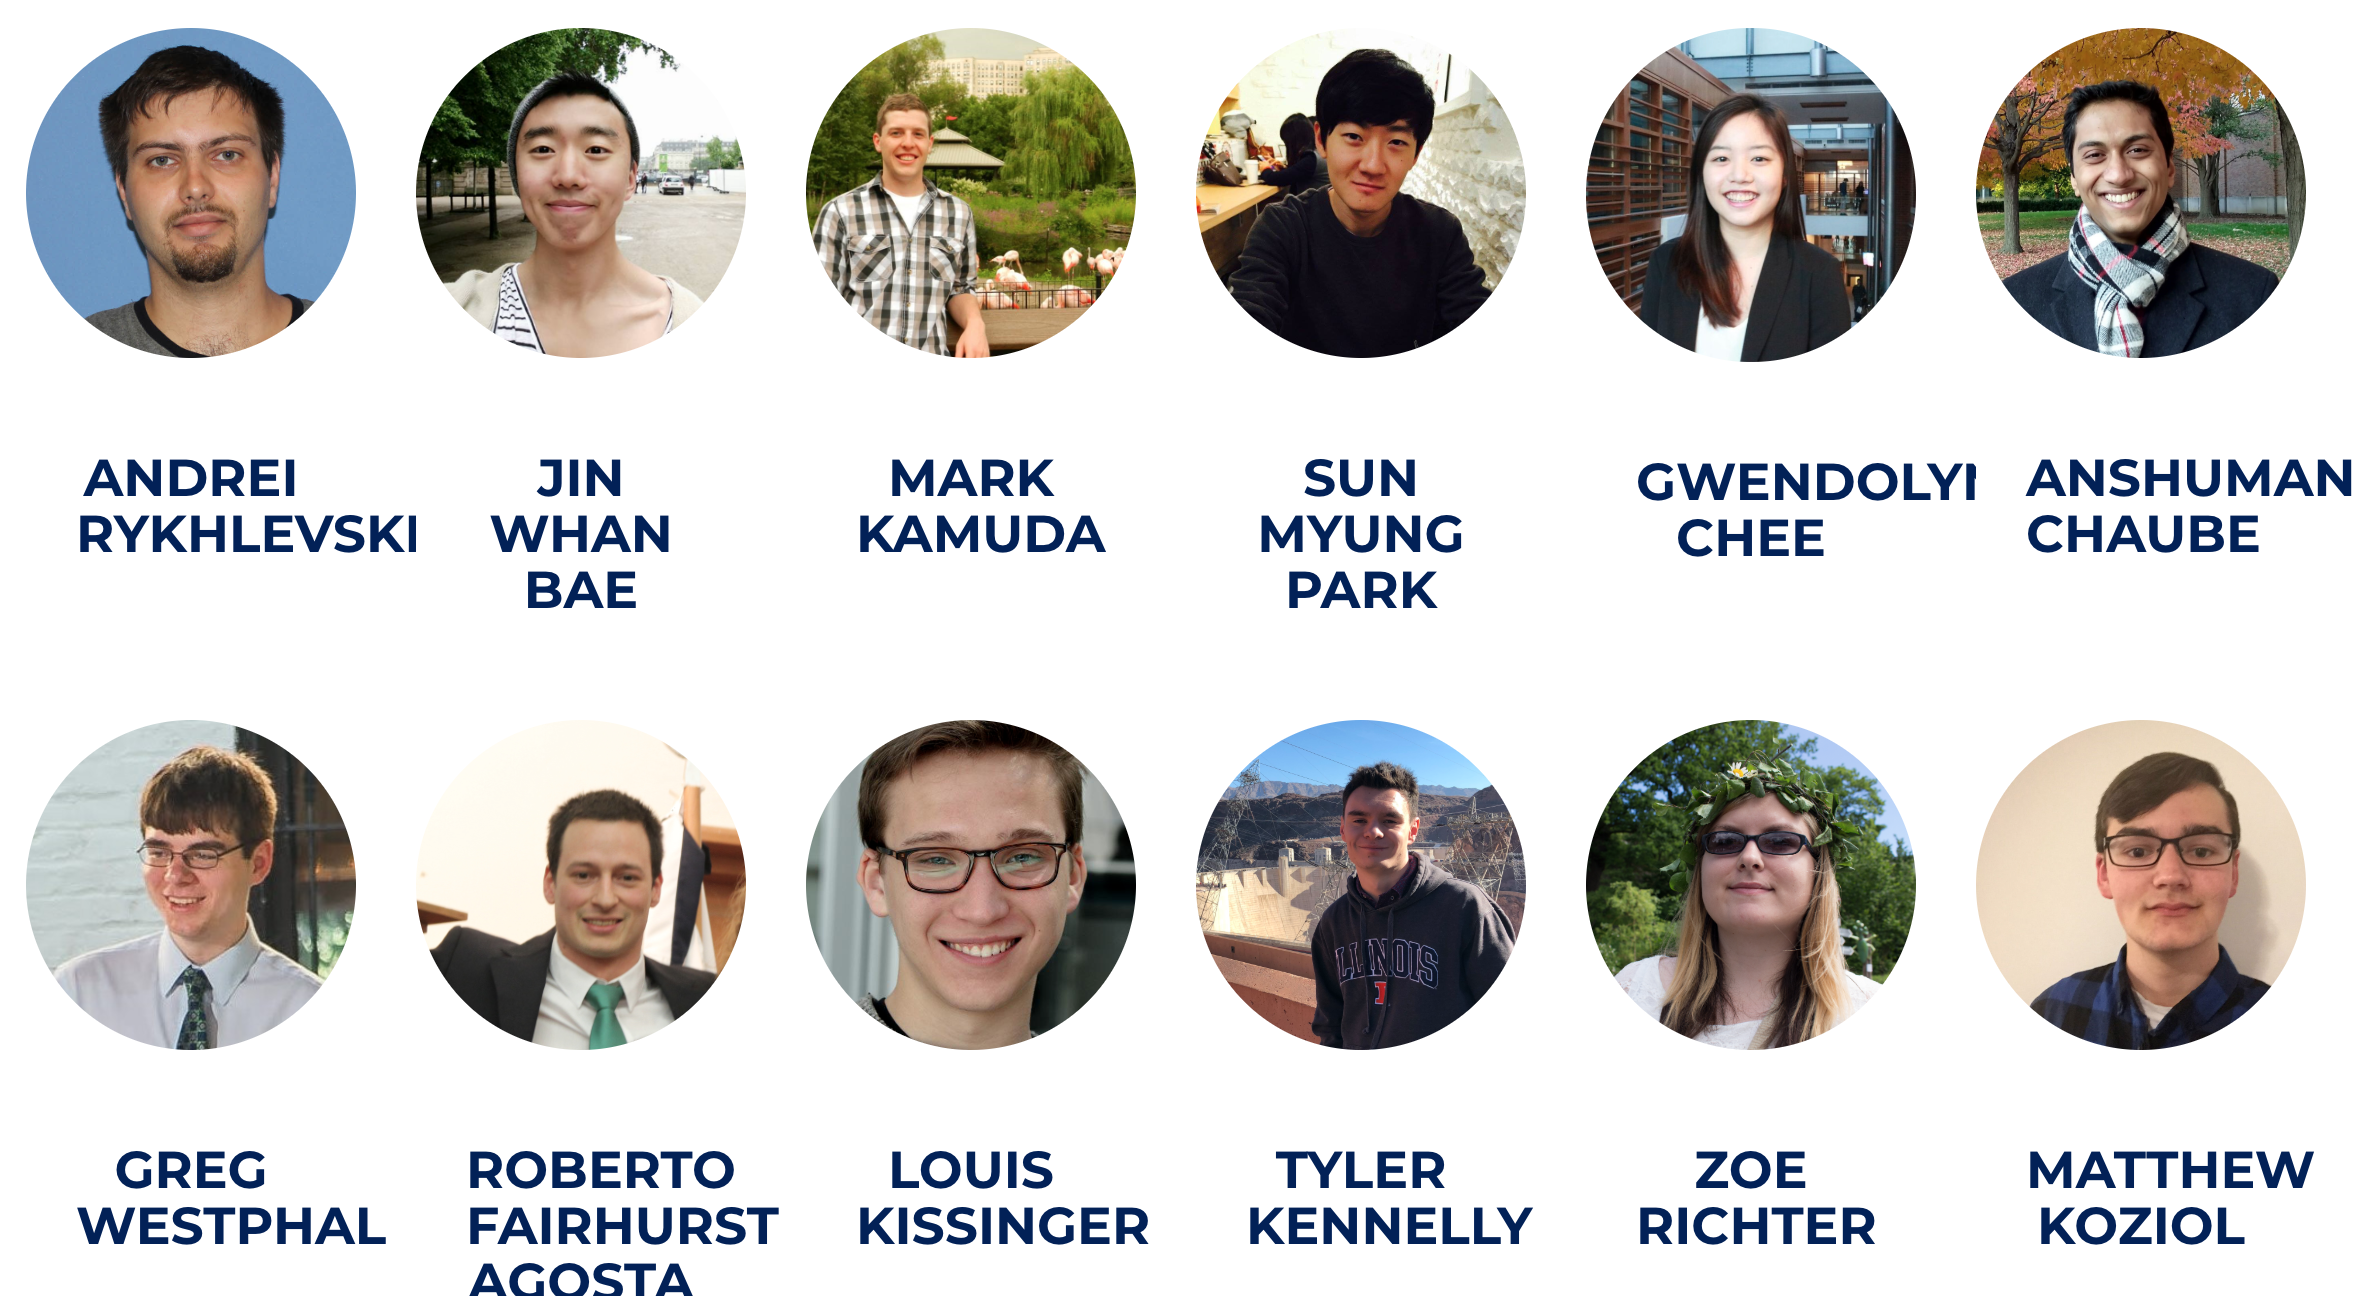
\includegraphics[width=\textwidth]{./images/arfc1.png}
                       \caption{Current undergraduate and graduate students.}
               \end{figure}            
\end{frame}
\begin{frame}
  \frametitle{Advanced Reactors and Fuel Cycles group (PI: Kathryn Huff)}
               \begin{figure}[t]
                \vspace*{-0.1in}
                
\includegraphics[width=\textwidth]{./images/arfc-alums.png}
                       \caption{Past ARFC Group members who contributed to this work.}
               \end{figure}            
\end{frame}

\begin{frame}
  \frametitle{Insights at Disparate Scales}
               \begin{figure}[t]
                \vspace*{-0.1in}
			\hspace*{-0.35in}
                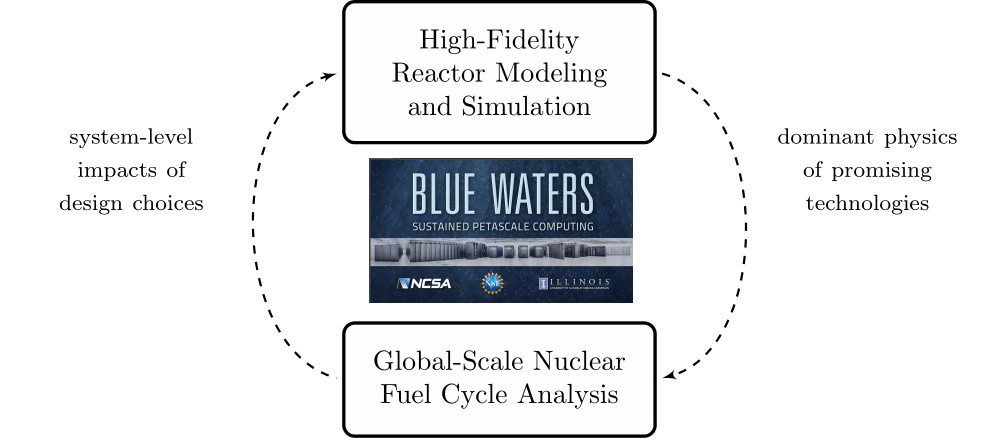
\includegraphics[height=0.5\textwidth]{./images/synergy.png}
               \end{figure}            
\end{frame}

\subsection{Molten Salt Reactors}

\begin{frame}
        \frametitle{Types of Molten Salt Reactors}
        \begin{block}{Stationary Fuel}
                \begin{itemize}
                        \item Prismatic graphite block with TRISO fuel and 
                                coolant channels (e.g. FHR DR, TMSR-SF1). Clean salt 
                                coolant.
                        \item Stationary TRISO pebble matrix (e.g. TMSR-SF)
                \end{itemize}

        \end{block}
        \begin{block}{Mobile Fuel}
                \begin{itemize}
                        \item Mobile solid fuel elements, such as pebbles. 
                                Clean salt coolant. (e.g. PB-FHR/Kairos)
                        \item Non-circulating fuel salt, ``can-type''. (e.g. Terrapower MCFR)
                        \item Circulating fuel salt ``pool-type''. (e.g. MSRE, MSBR, MSFR, 
                                Terrestrial MSR, TAP MSR, etc.)
                \end{itemize}
        \end{block}
\end{frame}

\begin{frame}
        \frametitle{Stationary Solid Fuel}
               \begin{figure}[t]
                \vspace*{-0.1in}
                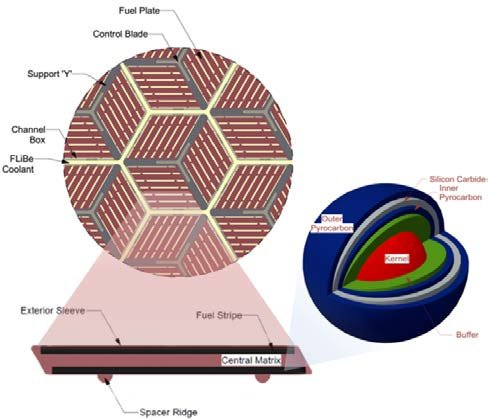
\includegraphics[height=0.5\textwidth]{./images/example-ahtr.png}
                       \caption{The \gls{AHTR} \cite{forsberg_fuel_2004} 
                       is an example of a fluoride salt cooled reactor 
                       design fueled by a \textbf{stationary}, \textbf{solid} 
                       prismatic graphite TRISO compacts, and cooled by clean fluoride salt.
                       Image source \cite{gentry_burnable_2015}. }
               \end{figure}            
\end{frame}

\begin{frame}
        \frametitle{Mobile Solid Fuel}
               \begin{figure}[t]
                \vspace*{-0.1in}
                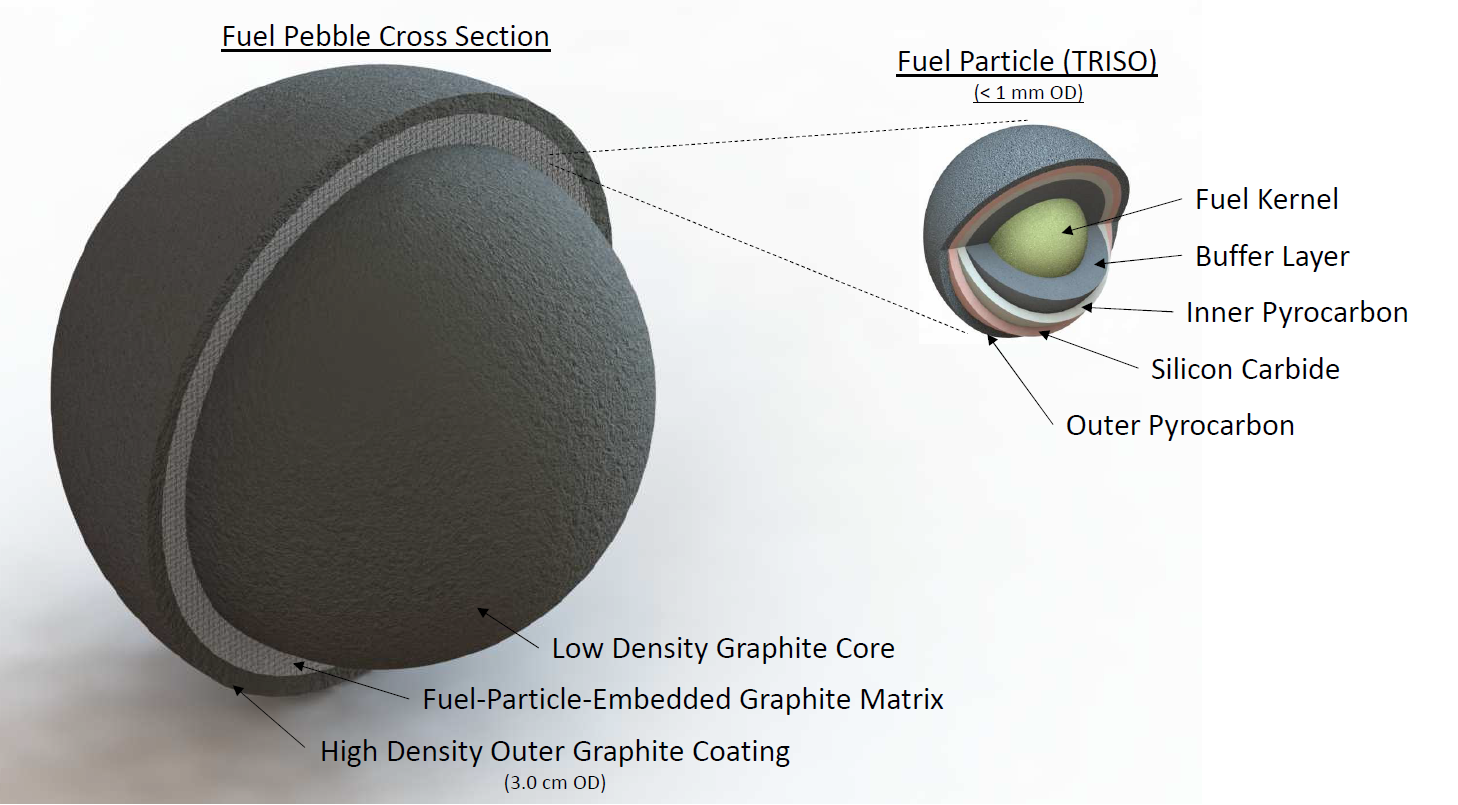
\includegraphics[height=0.2\textwidth]{./images/example-pbfhr-fuel.png}
                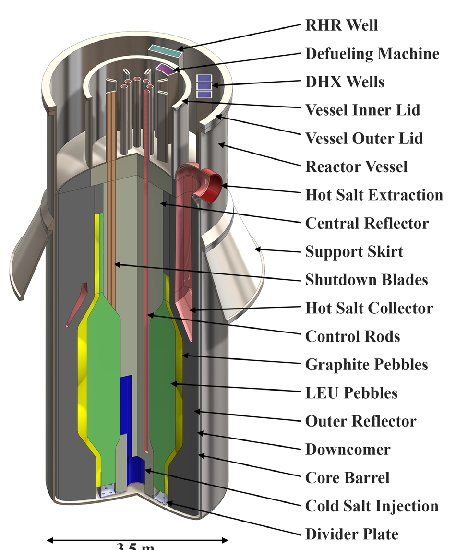
\includegraphics[height=0.4\textwidth]{./images/example-pbfhr-core.jpg}
                       \caption{The \gls{PBFHR} is an example reactor design 
                       fueled by \textbf{solid}, \textbf{mobile} graphite 
                       pebbles, with TRISO particles embedded in them. Image 
                       source \cite{andreades_technical_2014}.}
               \end{figure}            
\end{frame}

\begin{frame}
        \frametitle{Mobile, Non-Circulating, Liquid Fuel}
               \begin{figure}[t]
                \vspace*{-0.1in}
                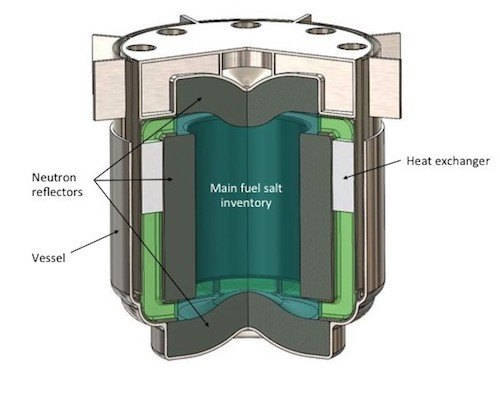
\includegraphics[height=0.5\textwidth]{./images/example-mcfr.jpg}
                       \caption{The \gls{MCFR} from TerraPower is an example 
                       reactor design with \textbf{liquid}, \textbf{mobile}, 
                       \textbf{non-circulating} chloride salt fuel. Image 
                       source \cite{terrapower_llc_mcfr_2018,doene_southern_2018}.}
               \end{figure}            
\end{frame}


\begin{frame}
        \frametitle{Mobile, Circulating, Liquid Fuel}
               \begin{figure}[t]
                \vspace*{-0.1in}
                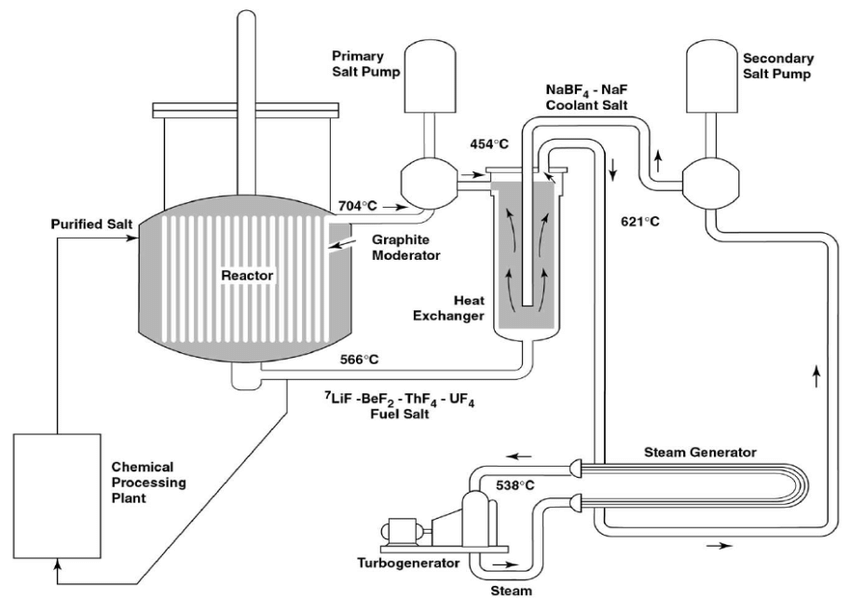
\includegraphics[height=0.5\textwidth]{./images/example-msbr.png}
                       \caption{The \gls{MSBR} \cite{robertson_conceptual_1971} is an example 
                       reactor design with \textbf{liquid}, \textbf{mobile}, 
                       \textbf{circulating} fluoride salt fuel, including 
                       breeding behavior due to varying channel shapes and 
                       sizes. Image 
                       source \cite{rosenthal_molten-salt_1970}.}
               \end{figure}            
\end{frame}

\begin{frame}
  \frametitle{Why Molten Salt Reactors?}
                  \vspace*{-0.1in}
              \begin{block}{Main advantages of liquid-fueled \glspl{MSR} \cite{elsheikh_safety_2013}}
               \begin{enumerate}
                \item High coolant temperature (600-750$^{\circ}$C).
                \item Various fuels can be used ($^{235}$U, $^{233}$U, Thorium, U/Pu).
                \item Increased inherent safety.
                \item High fuel utilization $\Rightarrow$ less nuclear waste generated.
                \item Online reprocessing and refueling.
               \end{enumerate}
               \end{block}
                  \vspace*{-0.1in}               
               \begin{block}{Main advantages of \gls{MSBR} \cite{robertson_conceptual_1971}}
               \begin{enumerate}
                \item Produces more fissile material than it consumes (breeding ratio 1.06).
                \item Thorium cycle limits plutonium and minor actinides.
                \item Could transmute spent fuel from existing \gls{NPP}.
               \end{enumerate}
               \end{block}

\end{frame}

\begin{frame}
  \frametitle{Challenges in Liquid-Fueled Reactor Simulation}
                  \vspace*{-0.05in}
               \begin{enumerate}
                \item Contemporary burnup codes cannot treat fuel movement.
                \item Neutron precursor locations drift before neutron emission.
                \item Operational and safety parameters change during reactor operation.
                \item Neutronics and thermal hydraulics are tightly interdependent.
               \end{enumerate}

           \begin{figure}[t]
                \vspace*{-0.05in}
			\hspace*{-0.2in}
                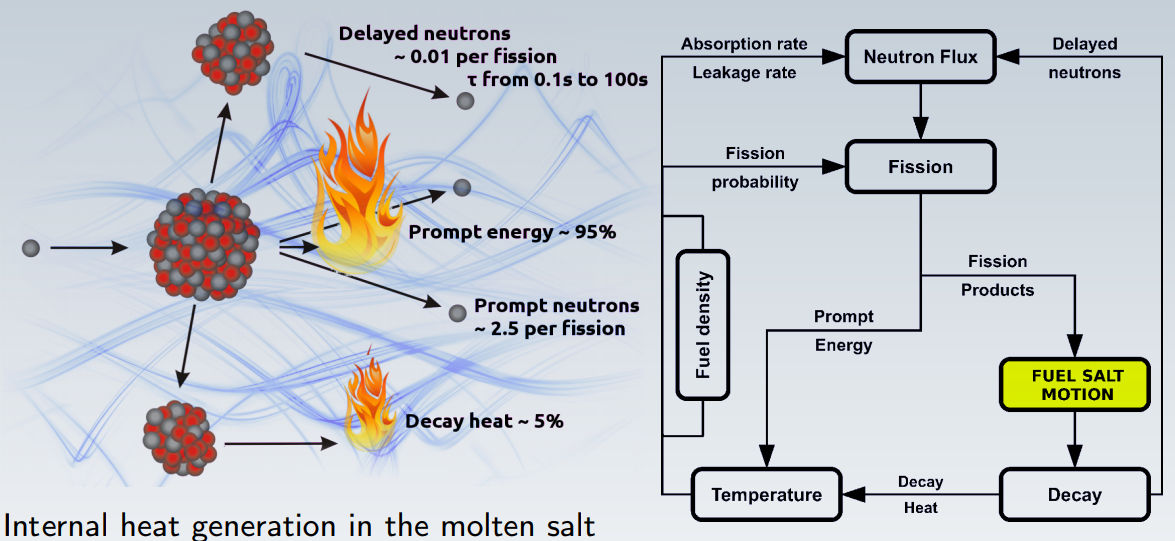
\includegraphics[height=0.47\textwidth]{./images/coupled_physics.png}
		\vspace*{-0.05in}
		\caption{Challenges in simulating \glspl{MSR} (Image courtesy of Manuele Aufiero, 2012).}
     	 \end{figure}               
\end{frame}

\begin{frame}
  \frametitle{Approaches}
                  \vspace*{-0.1in}
              \begin{block}{Point Reactor Kinetics \cite{huff_pyrk:_2015}}
                Only appropriate for stationary or nearly stationary fuels.
              \end{block}

              \begin{block}{Simulation of online reprocessing and depletion 
                      (SaltProc)\cite{rykhlevskii_arfc/saltproc:_2018,rykhlevskii_online_2017}}
               \begin{enumerate}
                \item Create high-fidelity full-core neutronics model of the 
                        core neutronics can be necessary for reducing 
                               compounding error.
                \item SaltProc wraps SERPENT monte carlo neutron transport for 
                        simulation of liquid fuel reprocessing.
                \item Enables day-to-day rsolution off neutronics and reprocessing modeling 
                        over many decades of depletion and fuel cycle performance.
               \end{enumerate}
               \end{block}

              \begin{block}{Multiphysics simulation of \gls{MSR} (Moltres)\cite{lindsay_introduction_2018}}
               \begin{enumerate}
                \item Steady-state and transient coupling of neutron fluxes, 
                        precursor drift, and thermal-hydraulics.
                \item Incorporates advective movement of delayed neutron precursors.
                \item 2D axisymmetric and 3D geometries supported.
               \end{enumerate}
               \end{block}

\end{frame}
